\section{Evaluation}
%TODO: Is there a good technical reason why every \absmachine machine
% should have exactly one large stateful atom as opposed to many small stateful atoms?
\label{s:eval}

\begin{table}[!t]
  \begin{scriptsize}
  \begin{tabular}{|p{0.1\textwidth}|p{0.35\textwidth}|}
    \hline
    Atom & Description \\
    \hline
    Write & Write packet field/constant into single state variable. \\
    \hline
    ReadAddWrite (RAW) & Add packet field/constant to state variable (OR) Write packet field/constant into state variable. \\
    \hline
    Predicated ReadAddWrite (RAW) & Execute RAW on state variable only if a predicate is true, otherwise leave unchanged. \\
    \hline
    IfElse ReadAddWrite (IfElseRaw) & Execute two separate RAWs: one each for when a predicate is true or false.\\
    \hline
    Subtract (Sub) & Same as IfElseRaw, but also allow subtracting a packet field/constant. \\
    \hline
    Nested Ifs (Nested) & Same as Sub, but with an additional level of nesting. \\
    \hline
    Paired updates (pairs) & Samed as Nested, but allow updates to a pair of state variables, where predicates can use both state variables. \\
    \hline
  \end{tabular}
  \end{scriptsize}
  \caption{Atoms used in evaluation.}
  \label{tab:templates}
\end{table}

\begin{table}[!t]
  \begin{scriptsize}
    \begin{tabular}{|p{0.1\textwidth}|p{0.3\textwidth}|p{0.03\textwidth}|}
  \hline
  Atom & Circuit & Depth \\
  \hline
  Write & 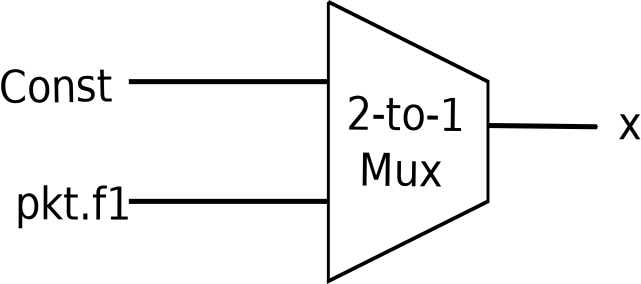
\includegraphics[width=0.2\textwidth]{rw.pdf} & 1 \\
  \hline
  ReadAddWrite (RAW) & 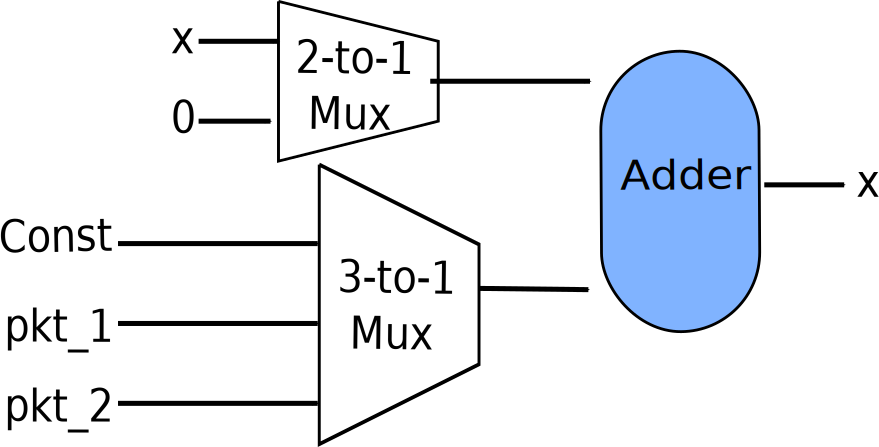
\includegraphics[width=0.2\textwidth]{raw.pdf} & 2\\
  \hline
  \pbox{0.1\textwidth}
  {Predicated\\
  ReadAddWrite (PRAW)} & \includegraphics[width=0.3\textwidth]{pred_raw.pdf}  & 3\\
  \hline
  \end{tabular}
\end{scriptsize}
\caption{Circuit depth (and hence propagation delay) increases with complexity of atoms.}
  \label{tab:circuit_depth}
\end{table}

\begin{table*}[!t]
  \begin{tabular}{|p{0.20\textwidth}|p{0.54\textwidth}|p{0.10\textwidth}|p{0.10\textwidth}|}
\hline
Algorithm & Stateful computation & Pipeline depth & Pipeline width \\
\hline
Bloom filter & \pbox{0.74\textwidth}{Set membership bit on every packet.} & & \\
\hline
Heavy Hitters~\cite{opensketch} & Increment Count-Min Sketch~\cite{cormode} on every packet. & & \\
\hline
Flowlets~\cite{flowlets} & Update saved next hop if flowlet threshold is exceeded. & & \\
\hline
RCP~\cite{rcp} & Accumulate RTT sum if RTT is under maximum allowable RTT. & & \\
\hline
Sampling & \pbox{0.74\textwidth}{Sample/Mark a packet if packet count reaches N; reset count to 0 at N.} & &\\
\hline
HULL~\cite{hull} & Update counter for virtual queue. & & \\
\hline
Adaptive Virtual Queue~\cite{avq} & & & \\
\hline
CONGA~\cite{conga} & \pbox{0.74\textwidth}{Update best path's utilization/id if we see a better path.\\
                                           Update best path utilization alone if it changes.}  & & \\
\hline
trTCM~\cite{trTCM} & & & \\
\hline
CoDel~\cite{codel} & & & \\
\hline
\end{tabular}
\caption{Data-plane algorithms}
\label{tab:algos}
\end{table*}

\begin{figure*}[!t]
  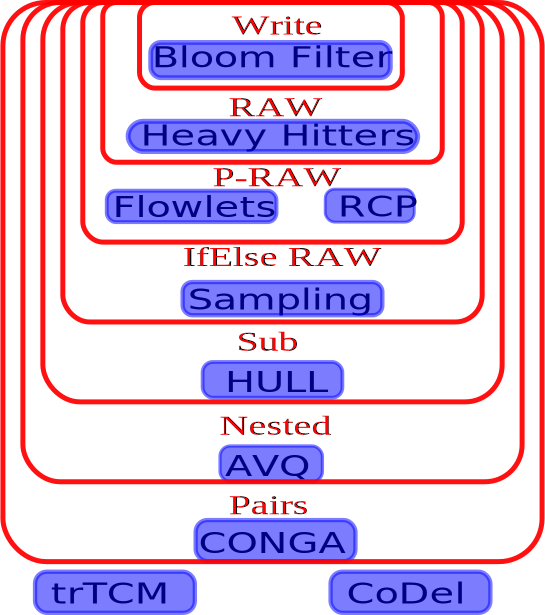
\includegraphics[width=\textwidth]{atom_hierarchy.pdf}
  \caption{Containment hierarchy of \absmachine machines and what data-plane algorithms each can implement.}
\label{fig:eval}
\end{figure*}

%10. Alvin's feedback: Write about our experience writing these programs. Similar to Steven Chong's PLDI paper.
To evaluate \pktlanguage, we express several well-known data-plane algorithms
(Table~\ref{tab:algos}) using \pktlanguage and determine if they are
implementable on different \absmachine machines that provide different stateful
atoms (Table~\ref{tab:templates}).

\subsection{Experimental procedure}
As mentioned before, we consider only stateful atoms by assuming stateless
codelets map one-to-one to stateless atoms for all \absmachine machines. For
simplicity, the stateful atoms only permit updates to state variables and
forbid packet field updates mixed in with these state updates.  Assuming the
\absmachine machine provides an atom to read a state variable\footnote{The
inability to read a state variable renders it powerless!}, such packet updates
can be treated as stateless operations in subsequent pipeline stages.

%Anirudh->Alvin: Is it clear now that each machine provides exactly one atom.
We also assume every \absmachine machine provides exactly one stateful atom.
Table~\ref{tab:templates} gradually increases the capability of this single
atom.  We designed the atoms in Table~\ref{tab:templates}, and the \absmachine
machines providing them, to form a containment hierarchy
(Figure~\ref{fig:eval}): each atom can express all data-plane algorithms that
its predecessor can.

We now consider every atom/\absmachine machine from Table~\ref{tab:templates},
and every data-plane algorithm from Table~\ref{tab:algos} to determine if each
algorithm is \textit{implementable} on a particular \absmachine machine. We
say an algorithm is implementable on a \absmachine machine, if every stateful
codelet within the data-plane algorithm can be mapped (\S\ref{ss:code_gen}) to
the single stateful atom provided by the \absmachine machine.

\subsection{Interpreting these results}
Figure~\ref{fig:eval} tells a network programmer if a particular data-plane
algorithm can be implemented at line rate, assuming the \absmachine machine
provides a particular stateful atom. For an ASIC engineer designing
programmable switching chips, the same figure describes the algorithms that are
implementable on a particular \absmachine machine. For instance, a \absmachine
machine with the paired updates atom can implement eight algorithms shown in
Figure~\ref{fig:eval}, while a machine with a simpler read-add-write atom can
implement only two.

These results will change as programmable switches evolve and network
programmers push chip boundaries with new algorithms.  The larger takeaway is
that programming in \pktlanguage allows us to rigorously determine if a
particular high-level algorithm is implementable at line rate on a particular
\absmachine machine. Conversely, it tells us if a particular \absmachine
machine suffices to implement a large number of algorithms.

\subsection{Compilation times}
